\documentclass[pdf]{beamer}

\usepackage{mathtools}
\usepackage{tikz}

\usepackage{listings}
\usepackage{color}

\newtheorem{principle}{Principle}
\newtheorem{proposition}{Proposition}
\definecolor{dkgreen}{rgb}{0,0.6,0}
\definecolor{gray}{rgb}{0.5,0.5,0.5}
\definecolor{mauve}{rgb}{0.58,0,0.82}

\lstset{frame=tb,
  language=Java,
  aboveskip=3mm,
  belowskip=3mm,
  showstringspaces=false,
  columns=flexible,
  basicstyle={\small\ttfamily},
  numbers=none,
  numberstyle=\tiny\color{gray},
  keywordstyle=\color{blue},
  commentstyle=\color{dkgreen},
  stringstyle=\color{mauve},
  breaklines=true,
  breakatwhitespace=true
  tabsize=3
}

\newcommand{\laplace}[1]{ \mathcal{L} \left\{ #1 \right\} }
\newcommand{\fourier}[1]{ \mathcal{F} \left\{ #1 \right\} }
\newcommand{\mellin}[1]{ \mathcal{M} \left\{ #1 \right\} }
\newcommand{\rld}[4]{ \left( \prescript{}{#1}{\mathcal{D}_{#2}^{#3}} #4 \right) }
\newcommand{\rli}[3]{ \left( I_{#1}^{#2} #3 \right) }
\newcommand{\der}[3]{ \frac{d^{#3}#1}{d#2^{#3}} }
\newcommand{\capder}[4]{ \left( \prescript{C}{#1}{\mathcal{D}_{#2}^{#3}} #4 \right) }
\newcommand{\fracdelta}[4]{ \left( \prescript{}{#1}{\Delta^{#2}_{#3} } #4 \right) }

\newcommand{\lra}{\longrightarrow}
\newcommand{\ra}{\rightarrow}
\newcommand{\lla}{\longleftarrow}
\newcommand{\la}{\leftarrow}

%Analysis
\newcommand{\Rl}{\mathbb{R}}
\newcommand{\Cplx}{\mathbb{C}}
\newcommand{\Itgr}{\mathbb{Z}}
\newcommand{\Ntrl}{\mathbb{N}}
\newcommand{\Ind}{\mathbbm{1}}
\newcommand{\Hlbt}{\mathcal{H}}
\newcommand{\im}{\operatorname{im}}

\mode<presentation>{}
\title{Accelerating Numerical Solutions to Fractional Differential Equations}
\subtitle{Adams Moulton Bashforth Method}
\author[Adam J. Gray]{Adam J. Gray\\{\small Supervised by: Dr Chris Tisdell}}
\institute{
	School of Mathematics and Statistics \\
	University of New South Wales
}

\begin{document}
\begin{frame}
	\titlepage
\end{frame}


\begin{frame}{Outline}
    \begin{itemize}
        \item Examine the Adams Moulton Bashforth method for a first order initial value problem.
        \item Examine a fractional Adams Moulton Bashforth method.
        \item Examine a parallel CPU based implementation of the scheme.
        \item Examine a parallel GPU based implementation of the scheme.
    \end{itemize}
\end{frame}

\begin{frame}{A first order problem}
We would like to solve the following initial value problem.
\begin{align*}
    \frac{d}{dx} y(x) = f(x,y)
\end{align*}
\begin{align*}
    y(0) = y_0
\end{align*}
This is equivalent to
\begin{align*}
    y(x) = y_0 + \int_0^x f(t, y(t))dt
\end{align*}
\end{frame}

\begin{frame}{The first step}
    Suppose we want to approximate the solution some small time-step $ h $ away from $ 0 $.
    \begin{align*}
        y(h) = y(0) + \int_0^h f(t, y(t)) dt
    \end{align*}
    Using a simple quadrature rule (trapezoidal) we could approximate the integral to get
    \begin{align*}
        y(h) = y(0) + \frac{h}{2} \left[ f(0, y(0)) + f(0, y(h)) \right]
    \end{align*}
\end{frame}

\begin{frame}{Predictor Approximation of y(h)}
    What if we approximate $ y(h) $ and use that value in the previous integral?
    We can do this by using the rectangle quadrature rule which
    gives us
    \begin{align*}
        \int_0^h f(t, y(t)) dt \approx h f(0, y(0))
    \end{align*}
    and so we could say
    \begin{align*}
        y^{P}(h) = y_0 + h f(0, y(0))
    \end{align*}
    and putting $y^{P}(h) $ in the equation before yields
    \begin{align*}
        y(h) = y(0) + \frac{h}{2} \left[ f(0, y(0)) + f(0, y^P(h)) \right]
    \end{align*}
\end{frame}

\begin{frame}{Iterating the process}
    The previous slides explained how to step forward one small time-step $ h $. We can now use the value calculated for $ y(h) $ as the \emph{initial value} and calculate $ y(2h) $.
    \begin{align*}
        y(2h) = y(h) + \frac{h}{2} \left[ f(h, y(h)), + f(2h, y^{P}(2h)) \right]
    \end{align*}
    with 
    \begin{align*}
        y^P(2h) = y(h) + hf(h, y(h)).
    \end{align*}
    We can restate this whole process iteratively:
    \begin{align*}
        y_{k+1} &= y_{k} + \frac{h}{2} \left[ f(x_k, y_k) + f(x_{k+1}, y_{k+1}^{P} ) \right] \\
        y^{P}_{k+1} &= y_k + hf(x_k, y_k)
    \end{align*}
\end{frame}

\begin{frame}{Is the only way of doing things?}
\begin{itemize}
    \item No! 
    
    \item There are lots of different schemes for numerically approximating the solutions to integer order initial value problems (RK3/4, Euler, Milne, etc).
    
    \item In fact we have hidden the Euler method inside this method. The Euler method basically puts some small but non-zero $ h $ into the first principles definition of the derivative and solves from there.
    
\end{itemize}

\end{frame}

\begin{frame}{Key Computational Points of this Method}
\begin{itemize}
    \item It's numerically stable for reasonable choices of $ f $.
    \item It's convergent of order $ 2 $ in the sense that 
    \begin{align*}
        \max_{j=0,1,...,N} | y(t_j) - y_j | = O(h^2) 
    \end{align*}
    \item The computational complexity is $ O(N) $ (linear time).
\end{itemize}
 
\end{frame}

\begin{frame}{The Fractional Problem}
    We wish to solve a fractional initial value problem of the form
    \begin{align*}
        \capder{0}{x}{\alpha}{y}(x) = f(x,y)
    \end{align*}
    along with initial conditions
    \begin{align*}
        y(0) = y_0^{(k)} & & 0 \leq k \leq \lceil \alpha \rceil - 1
    \end{align*}
    \hrulefill
    \begin{align*}
        \capder{0}{x}{\alpha}{y}(x) = \frac{1}{\Gamma( \lceil \alpha \rceil - \alpha)} \int_{0}^{x} \frac{\frac{d^{\lceil \alpha \rceil}}{dt^{\lceil \alpha \rceil}} y(t)}{(x-t)^{\lceil \alpha \rceil - \alpha + 1}}dt
    \end{align*}
\end{frame}

\begin{frame}{Equivalent Integral Equation}
The initial value problem
    \begin{align*}
        \capder{0}{x}{\alpha}{y}(x) = f(x,y)
    \end{align*}
    along with initial conditions
    \begin{align*}
        y(0) = y_0^{(k)} & & 0 \leq k \leq \lceil \alpha \rceil - 1
    \end{align*}
    is equivalent to the integral equation
    \begin{align*}
        y(x) = \sum_{k = 0}^{\lceil \alpha \rceil - 1} y_0^{(k)} \frac{x^k}{k!} + \frac{1}{\Gamma(\alpha)} \int_0^x (x - t)^{\alpha - 1}f(t,y(t))dt
    \end{align*}
\end{frame}

\begin{frame}{The Fractional Case}
    \begin{align*}
    y_{k+1} &= \sum_{j=0}^{\lceil \alpha \rceil - 1} y_{0}^{(j)} \frac{x^j_{k+1}}{j!} + \\
    & \frac{1}{\Gamma(\alpha)} \left( \sum_{j=0}^k a_{j,k+1} f(x_j,y_j) + a_{k+1,k+1}f(x_{k+1}, y_{k+1}^P )\right) \\
    y_{k+1}^P &= \sum_{j=0}^{\lceil \alpha \rceil - 1} \frac{x^{j}_{k+1}}{j!} y_{0}^{(j)} + \frac{1}{\Gamma(\alpha)} \sum_{j=0}^{k} b_{j,k+1} f(x_j, y_j).
\end{align*}

\end{frame}

\begin{frame}{Coefficients}
\begin{align*}
    a_{j,k+1} &= \frac{h^\alpha}{\alpha(\alpha+1)} \times
    \begin{cases}
        (k^{\alpha+1}-(k-\alpha)(k+1)^\alpha) & \text{ if } j = 0 \\
        ((k-j+2)^{\alpha + 1} + (k-j)^{\alpha+1} - 2(k-j+1)^{\alpha+1}) & \text{ if } 1 \leq j \leq k \\
        1 & \text{ if } j = k + 1.
    \end{cases} \\
    b_{j,k+1} &= \frac{h^\alpha}{\alpha} \left( (k+1-j)^\alpha - (k-j)^\alpha \right).
\end{align*}
\end{frame}

\begin{frame}{Parallel Approach}
\resizebox{300pt}{!}{
%AMB Y processing diagram

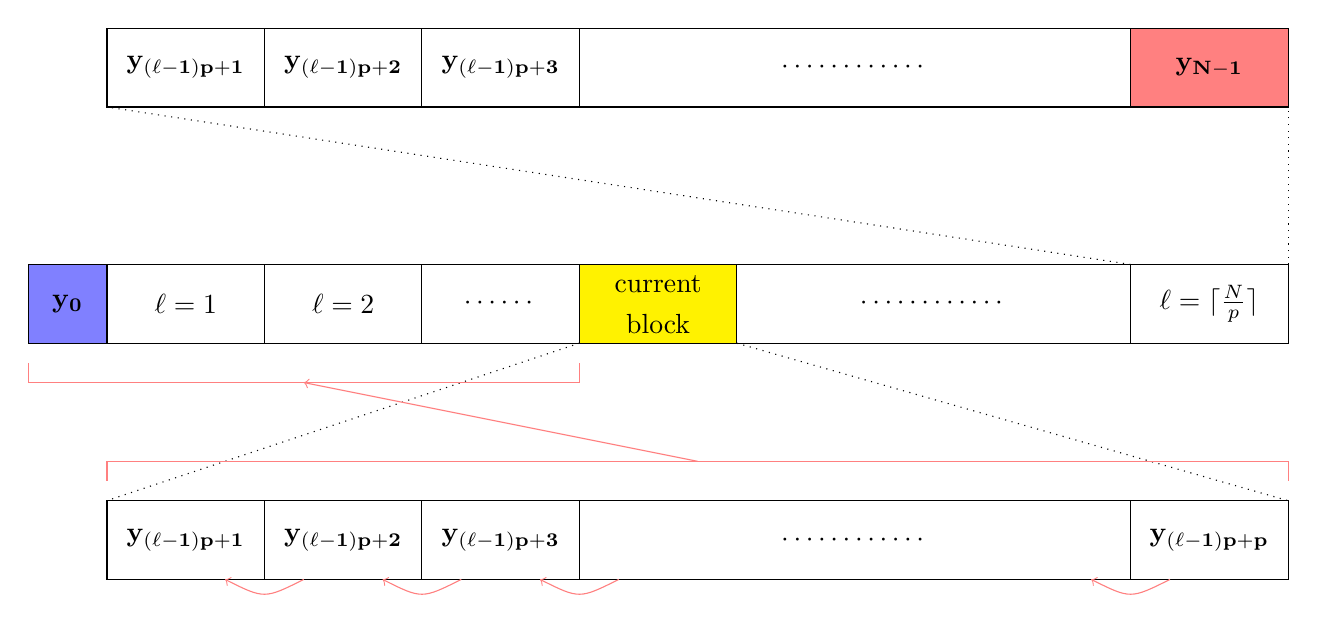
\begin{tikzpicture}
    \filldraw[fill=blue!50] (-1,0) rectangle (0,1);
    \draw (0,0) -- (0,1);
    \draw (-0.5,0.5) node { $ \mathbf{y_0} $ };
    \draw (-1,0) -- (15,0) -- (15, 1) -- (-1, 1) -- cycle;
    \draw (2,0) -- (2,1);
    \draw (4,0) -- (4,1);
    \draw (1,0.5) node { $ \ell = 1 $ };
    \draw (3,0.5) node { $ \ell = 2 $ };
    \draw (5,0.5) node { $ \cdots \cdots $ };
    \draw (6,0) -- (6,1);
    \draw (8,0) -- (8,1);
    \draw (10.5,0.5) node { $ \cdots \cdots \cdots \cdots  $ };
    \draw (13,0) -- (13,1);
    \draw (14,0.5) node { $ \ell = \lceil \frac{N}{p} \rceil $ };
    \filldraw[fill=yellow] (6,0) rectangle (8,1);
    \draw (7,0.75) node { current };
    \draw (7,0.25) node { block };
    \draw [dotted] (6,0) -- (0,-2);
    \draw [dotted] (8,0) -- (15,-2);
    \draw (0,-2) -- (15,-2) -- (15,-3) -- (0,-3) -- cycle;
    \draw (2,-3) -- (2,-2);
    \draw (4,-3) -- (4,-2);
    \draw (6,-3) -- (6,-2);
    \draw (13,-3) -- (13,-2);
    \draw (1,-2.5) node { $ \mathbf{ y_{(\ell - 1) p + 1} } $ };
    \draw (3,-2.5) node { $ \mathbf{ y_{(\ell - 1) p + 2} } $ };
    \draw (5,-2.5) node { $ \mathbf{ y_{(\ell - 1) p + 3} } $ };
    \draw (9.5, -2.5) node { $ \cdots \cdots \cdots \cdots $ };
    \draw (14,-2.5) node { $ \mathbf{ y_{(\ell - 1) p + p} } $ };
    \draw [dotted] (13,1) -- (0,3);
    \draw [dotted] (15,1) -- (15,3);
    \draw (0,3) -- (15,3) -- (15,4) -- (0,4) -- cycle;
    \draw (2,3) -- (2,4);
    \draw (4,3) -- (4,4);
    \draw (6,3) -- (6,4);
    \filldraw[fill=red!50] (13,3) rectangle (15,4);
    \draw (13,3) -- (13,4);
    \draw (1,3.5) node { $ \mathbf{ y_{(\ell-1)p + 1} } $ };
    \draw (3,3.5) node { $ \mathbf{ y_{(\ell-1)p + 2} } $ };
    \draw (5,3.5) node { $ \mathbf{ y_{(\ell-1)p + 3} } $ };
    \draw (9.5,3.5) node { $ \cdots \cdots \cdots \cdots $ };
    \draw (14,3.5) node { $ \mathbf{ y_{N-1} } $ };
    \draw [color=red!50, arrows={->}] (13.5,-3) .. controls (13,-3.25) .. (12.5,-3); 
    \draw [color=red!50, arrows={->}] (6.5,-3) .. controls (6,-3.25) .. (5.5,-3); 
    \draw [color=red!50, arrows={->}] (4.5,-3) .. controls (4,-3.25) .. (3.5,-3);    
    \draw [color=red!50, arrows={->}] (2.5,-3) .. controls (2,-3.25) .. (1.5,-3);
    \draw [color=red!50] (-1,-0.25) -- (-1,-0.5) -- (6,-0.5) -- (6,-0.25);
    \draw [color=red!50] (0,-1.75) -- (0,-1.5) -- (15,-1.5) -- (15,-1.75);
    \draw [color=red!50, arrows={->}] (7.5,-1.5) -- (2.5, -0.5);
\end{tikzpicture}

}
\end{frame}
\begin{frame}{Parallel Formulation}
We can requite the previous equations in the form
\begin{align*}
y_{j+1}^P = I_{j+1} + h^\alpha H_{j,\ell}^P + h^\alpha L_{j,\ell}^P
\end{align*}
and
\begin{align*}
y_{j+1} = I_{j+1} + h^{\alpha} H_{j,\ell} + h^\alpha L_{j,\ell}
\end{align*}
\end{frame}
\begin{frame}{Parallel Formulation}
\begin{align*}
I_{j+1} & := \sum_{k=0}^{\lceil \alpha \rceil -1} \frac{x_{j+1}^k}{k!} y_0^{(k)} \\
H^P_{j,\ell} & := \sum_{k=0}^{(\ell-1)p} b_{j-k} f(x_k, y_k) \\
L_{j,\ell}^P & := \sum_{k=(\ell-1)p+1}^{j} b_{j-k} f(x_k,y_k) \\
H_{j,\ell} & := c_j f(x_0, y_0) + \sum_{k=1}^{(\ell - 1)p} a_{j-k}f(x_k, y_k) \\
L_{j,\ell} & := \sum_{k=(\ell-1)p + 1}^j a{j-k} f(x_k, y_k) + \frac{f(x_{j+1}, y^P_{j+1})}{\Gamma(\alpha + 2.)}
\end{align*}
\end{frame}

\begin{frame}{Task Flow (in a single block)}
\resizebox{200pt}{!}{
%PID Controller Closed Loop Diagram.
\begin{tikzpicture} 
    \draw (10,20) -- (13,20) -- (13, 19) -- (10, 19) -- cycle;
    \draw (11.5,19.5) node { Block Start };
    \draw (11.5, 19) -- (11.5, 18);
    \draw (4.5, 18) -- (19.5, 18);
    \draw [->] (4.5, 18) -- (4.5, 17);
    \draw [->] (7.5, 18) -- (7.5, 17);
    \draw [->] (10.5, 18) -- (10.5, 17);
    \draw [->] (11.5, 18) -- (11.5, 13) -- (10, 13);
    \draw (3.75, 17) -- (5.25, 17) -- (5.25, 15.5) -- (3.75, 15.5) -- cycle;
    \draw (6.75, 17) -- (8.25, 17) -- (8.25, 15.5) -- (6.75, 15.5) -- cycle;
    \draw (9.75, 17) -- (11.25, 17) -- (11.25, 15.5) -- (9.75, 15.5) -- cycle;
    \draw (8.5, 12.25) -- (10, 12.25) -- (10,13.75) -- (8.5, 13.75) -- cycle;
    \draw (7.5, 14.5) -- (10.5, 14.5);
    \draw [->] (4.5, 15.5) -- (4.5, 4.25) -- (8.5, 4.25);
    \draw (7.5, 14.5) -- (7.5, 15.5);
    \draw (10.5, 14.5) -- (10.5, 15.5);
    \draw (7.5, 15.5) -- (7.5, 10);
    \draw [->] (7.5, 10) -- (8.5, 10);
    \draw (8.5, 9.25) -- (8.5, 10.75) -- (10, 10.75) -- (10, 9.25) -- cycle;
    \draw [->] (9.25, 12.25) -- (9.25, 10.75);
    \draw [->] (9.25, 9.25) -- (9.25, 8);
    \draw (8.5, 8) -- (10, 8) -- (10, 6.5) -- (8.5, 6.5) -- cycle ;
    \draw [->] (9.25, 6.5) -- (9.25, 5);
    \draw (8.5, 5) -- (8.5, 3.5) -- (10, 3.5) -- (10, 5) -- cycle;
    \draw [->] (18.5, 18) -- (18.5, 17);
    \draw [->] (15.5, 18) -- (15.5, 17);
    \draw [->] (12.5, 18) -- (12.5, 17);
    \draw (11.75, 17) -- (13.25, 17) -- (13.25, 15.5) -- (11.75, 15.5) -- cycle;
    \draw (14.75, 17) -- (16.25, 17) -- (16.25, 15.5) -- (14.75, 15.5) -- cycle;
    \draw (17.75, 17) -- (19.25, 17) -- (19.25, 15.5) -- (17.75, 15.5) -- cycle;
    \draw [->] (12.5, 15.5) -- (12.5, 4.25) -- (16.5, 4.25);
    \draw [->] (19.5, 18) -- (19.5, 13) -- (18, 13);
    
    
    \draw (15.5, 14.5) -- (18.5, 14.5);
    \draw [->] (12.5, 15.5) -- (12.5, 4.25) -- (16.5, 4.25);
    \draw (15.5, 14.5) -- (15.5, 15.5);
    \draw (18.5, 14.5) -- (18.5, 15.5);
    \draw (15.5, 15.5) -- (15.5, 10);
    \draw [->] (15.5, 10) -- (16.5, 10);
    \draw (16.5, 9.25) -- (16.5, 10.75) -- (18, 10.75) -- (18, 9.25) -- cycle;
    \draw [->] (17.25, 12.25) -- (17.25, 10.75);
    \draw [->] (17.25, 9.25) -- (17.25, 8);
    \draw (16.5, 8) -- (18, 8) -- (18, 6.5) -- (16.5, 6.5) -- cycle ;
    \draw [->] (17.25, 6.5) -- (17.25, 5);
    \draw (16.5, 5) -- (16.5, 3.5) -- (18, 3.5) -- (18, 5) -- cycle;
    \draw (16.5, 12.25) -- (18, 12.25) -- (18,13.75) -- (16.5, 13.75) -- cycle;
    \draw [color=red, arrows={->}] (10, 4.25) -- (12,4.25) -- (12, 13) -- (16.5, 13);
    \draw (4.5, 16.25) node { $ H $ };
    \draw (5, 15.75) node[color=red]  { $ 1 $ };
    
    \draw (7.5, 16.25) node { $ I $ };
    \draw (8, 15.75) node[color=red]  { $ 1 $ };
    
    \draw (10.5, 16.25) node { $ H_p $ };
    \draw (11, 15.75) node[color=red]  { $ 1 $ };
    
    \draw (9.25, 13) node { $ L_p $ };
    \draw (9.75, 12.5) node[color=red] { $ 1 $ };
    
    \draw (9.25, 10) node { $ S_p $ };
    \draw (9.75, 9.5) node[color=red] { $ 1 $ };
    
    \draw (9.25, 7.25) node { $ L $ };
    \draw (9.75, 6.75) node[color=red] { $ 1 $ };
    
    \draw (9.25, 4.25) node { $ L $ };
    \draw (9.75, 3.75) node[color=red] { $ 1 $ };
    
    
    
    \draw (12.5, 16.25) node { $ H $ };
    \draw (13, 15.75) node[color=red]  { $ 2 $ };
    
    \draw (15.5, 16.25) node { $ I $ };
    \draw (16, 15.75) node[color=red]  { $ 2 $ };
    
    \draw (18.5, 16.25) node { $ H_p $ };
    \draw (19, 15.75) node[color=red]  { $ 2 $ };
    
    \draw (17.25, 13) node { $ L_p $ };
    \draw (17.75, 12.5) node[color=red] { $ 2 $ };
    
    \draw (17.25, 10) node { $ S_p $ };
    \draw (17.75, 9.5) node[color=red] { $ 2 $ };
    
    \draw (17.25, 7.25) node { $ L $ };
    \draw (17.75, 6.75) node[color=red] { $ 2 $ };
    
    \draw (17.25, 4.25) node { $ L $ };
    \draw (17.75, 3.75) node[color=red] { $ 2 $ };
    
    \draw [->] (17.25, 3.5) -- (17.25, 2) -- (11.5, 2) -- (11.5, 1);
    
    \draw (10,1) -- (13,1) -- (13, 0) -- (10, 0) -- cycle;
    \draw (11.5,0.5) node { Block End };
\end{tikzpicture}

}
\end{frame}
\begin{frame}{Is this parallelization reasonable?}
\begin{principle}[Amdahl]
Let $ P $ be the proportion of a computation which can be parallelized in a given progress. Then the speedup given by
$ Q $ cores is
\begin{align*}
	S(Q) = \frac{1}{(1-P)+\frac{P}{Q}}
\end{align*}

\end{principle}

\begin{definition}[Amdahl Efficiency]
\label{def:amdahl_efficient}
    Let $ S(N,Q) $ represent the parallel speedup for a problem with input size $ N $ and executed with $ Q $ cores.
    Then we define the Amdahl efficiency of parallel scheme as 
    \begin{align*}
        E(Q) = \lim_{N \lra \infty} \frac{S(N, Q)}{Q}.
    \end{align*}
    Further we say that a parallel scheme is Amdahl efficient with respect to its serial counterpart if $ E(Q) = 1 $.
\end{definition}
\end{frame}


\begin{frame}
\begin{proposition}
The parallel Adams Moulton Bashforth scheme is Amdahl efficient with respect to its serial counterpart.
\end{proposition}
\begin{proof}
We present the parallelizable fraction of computation in each block of variables in the following table. The order column represents the number of \emph{multiply-add} operations per task.
\end{proof}
\resizebox{300pt}{!}{
\begin{tabular}[ht]{|c|c|c|c|}
\hline
Task        & Computational Complexity  & Number of Variables per Block     & Total Complexity \\ \hline
$ H $       & $ O(\ell p ) $            & $ p $                             & $ O(\ell p^2) $ \\ \hline
$ H_p $     & $ O(\ell p ) $            & $ p $                             & $ O(\ell p^2) $ \\ \hline
$ I $       & $ O( \alpha ) $           & $ p $                             & $ O(p) $ \\ \hline \hline          
$ L $       & $ O( p ) $                & $ p $                             & $ O(p^2) $ \\ \hline
$ L_p $     & $ O( p ) $                & $ p $                             & $ O(p^2) $ \\ \hline
\end{tabular}
}
\end{frame}
\begin{frame}
In each block $ H $, $ H_p $ and $ I $ can be computed in parallel across all variables in the block. For the purposes of simplicity we assume that the tasks $ L $ and $ L_p $ must all be computed in serial across all variables in a block. This means that in the $ \ell$-th block the non-parallelizable fraction of computation is
\begin{align*}
    \overline{P}_{block}(\ell) \sim \frac{2p^2}{2p^2(\ell + 1) } \sim \frac{1}{\ell}
\end{align*}

The amount of computation in the $ \ell$-th block is $ O(\ell p^2) $ and there are $ K \approx \frac{N}{p} $ blocks in the total computation. This means that the total amount of computation is
\begin{align*}
    \sum_{\ell=1}^{K} \ell p^2 \sim \frac{K^2p^2}{2}
\end{align*}
and by taking a weighted average sum, the total fraction of non-parallelizable computation is
\begin{align*}
    \label{eq:tot_par_c}
    \overline{P}_{total} \sim \sum_{\ell = 1}^{K} \frac{2\ell p^2}{K^2 \ell p^2} = \frac{2}{K} = \frac{2p}{N}.
\end{align*}
\end{frame}
\begin{frame}
Noticing the fact that the computation in the task $ I $ is insignificant compared to $ H $ and $ H_p $ we would suppose using $ Q = 2p $ cores would be in some sense optimal. Applying Amdahl's principle with the result in \ref{eq:tot_par_c} and with $ Q = 2p $ we get 
\begin{align*}
    S(N, Q) &= S(N, 2p) \\
    &\sim \frac{1}{(\frac{2p}{N}) + \frac{1-\frac{2p}{N}}{2p} } \\
\end{align*}
then letting $ N \lra \infty $ we get
\begin{align*}
    E(p) = \lim_{N \lra \infty} \left(\frac{1}{(\frac{2p}{N}) + \frac{1-\frac{2p}{N}}{2p} } \right) \slash p = 1.
\end{align*}
\end{frame}

\begin{frame}{Practical Experimentation}
I solved the initial value problem being discussed with $ \alpha = \frac{1}{2} $ and $ y(0) = 1 $ over the interval $ [0, 1] $ using a C\# implementation of the above algorithm.
\end{frame}
\begin{frame}{Practical Experimentation}
\begin{figure}[H]
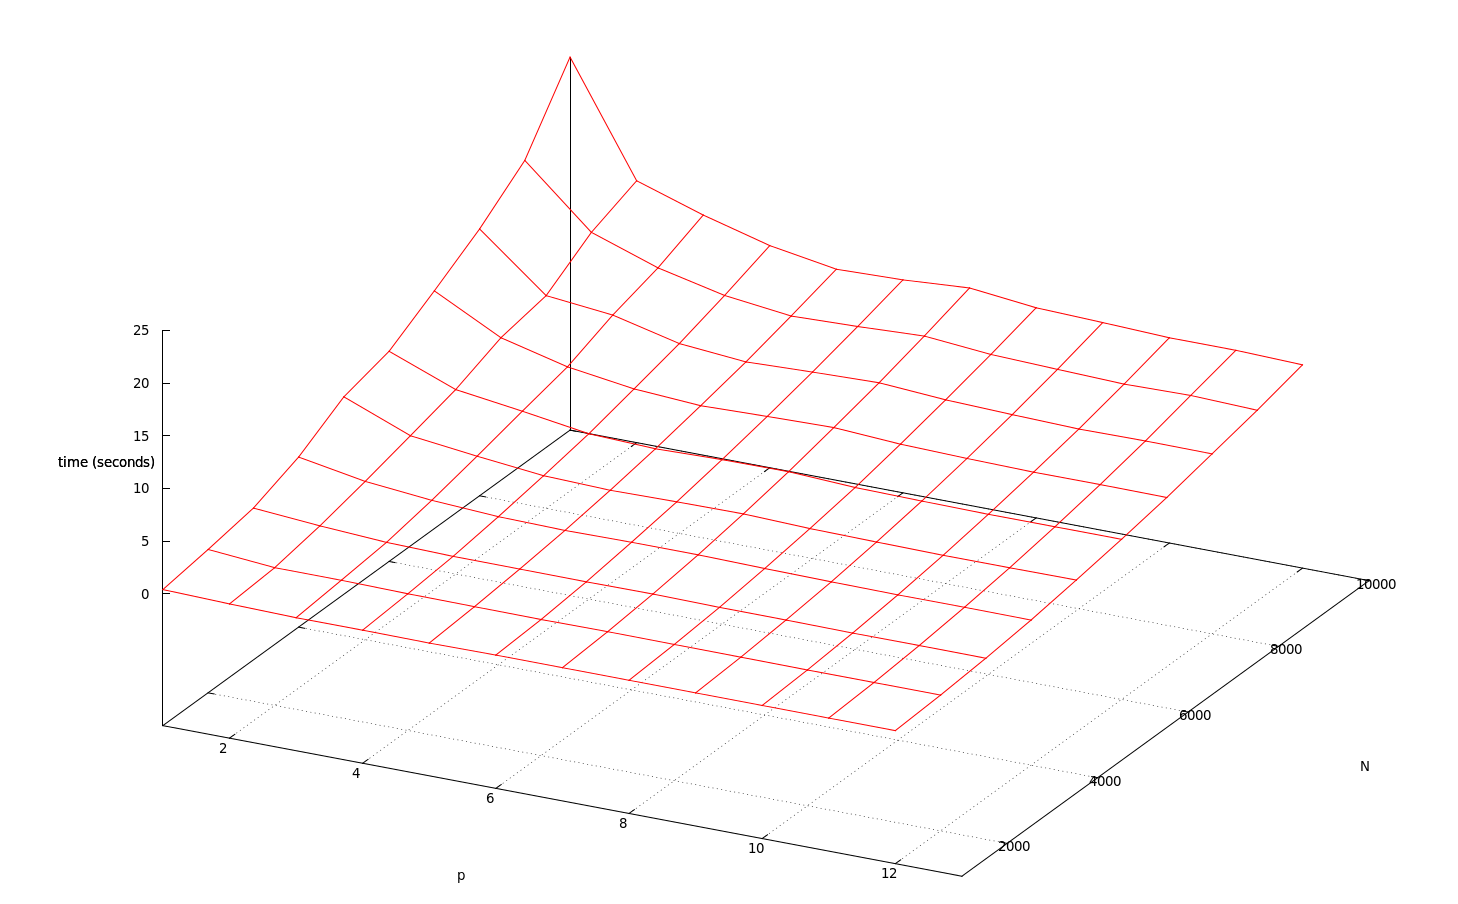
\includegraphics[scale = 0.2]{../images/Dot_Net_Performance_No_Label}
\caption{Average runtime of the scheme for different values of $ p $ and $ N $}
\label{fig:mono_performance_surface}
\end{figure}
\end{frame}

\begin{frame}{Redesigning the Algorithm for CUDA}
    Instead of trying to compute multiple variables in parallel we just return to the original (single threaded) formulation of the scheme and compute the large sums in parallel. 
        \begin{align*}
    y_{k+1} &= \sum_{j=0}^{\lceil \alpha \rceil - 1} y_{0}^{(j)} \frac{x^j_{k+1}}{j!} + \\
    & \frac{1}{\Gamma(\alpha)} \left( \sum_{j=0}^k a_{j,k+1} f(x_j,y_j) + a_{k+1,k+1}f(x_{k+1}, y_{k+1}^P )\right) \\
    y_{k+1}^P &= \sum_{j=0}^{\lceil \alpha \rceil - 1} \frac{x^{j}_{k+1}}{j!} y_{0}^{(j)} + \frac{1}{\Gamma(\alpha)} \sum_{j=0}^{k} b_{j,k+1} f(x_j, y_j).
\end{align*}
\end{frame}


\begin{frame}{Quick Notes for CUDA}
\begin{itemize}
    \item CUDA is particularly good for SIMD type computations (same instructions multiple data). We also refer to this as data parallelism. (We have a large amount of that in this particular case)
    \item We by calling a function in CUDA we can actually be invoking 1000s of instances of the function. 
    \item Each instance is passed \emph{grid reference} so it knows what part of the data to work on. Groups of instances (up to 1024) can do some limited communication and perform a small set of atomic operations on shared memory. This allows us add up the sub results.
\end{itemize}
\end{frame}

\begin{frame}{Practical Experimentation}
I solved the same initial value problem as I did in the C\# case. 
\begin{figure}[H]
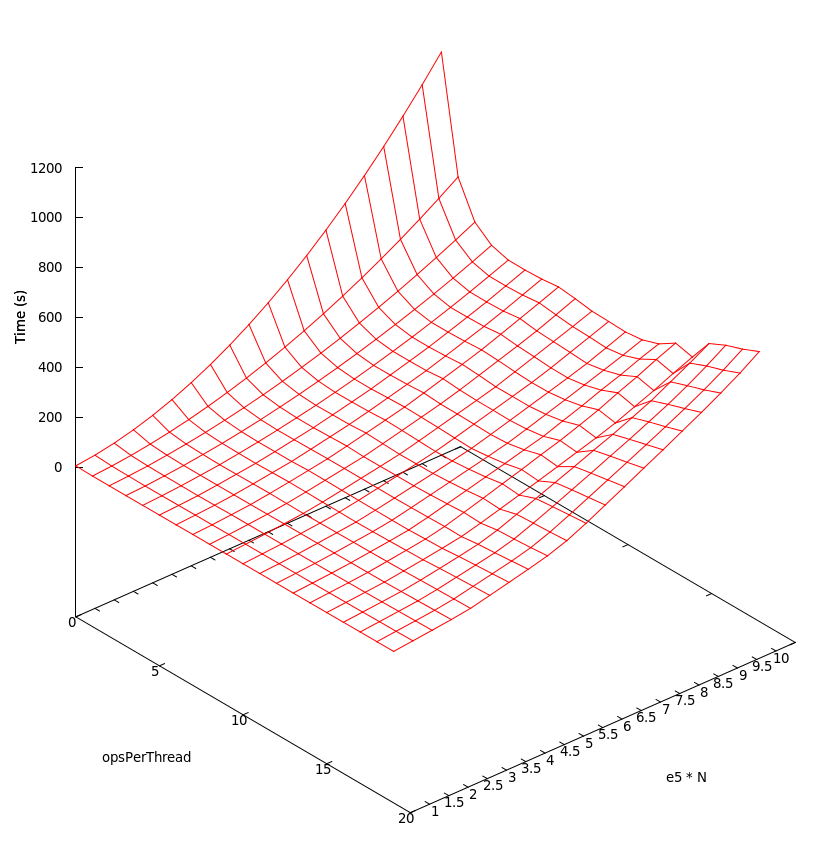
\includegraphics[scale = 0.2]{../images/CUDA_Performance_No_Label}
\caption{Runtime for the scheme for various values of opsPerThread and N.}
\label{fig:cuda_performance_surface}
\end{figure}

\end{frame}

\begin{frame}{Lets play...}
Solution to the relaxation oscillation equation for $ \alpha \in [0.5, 2] $.
\begin{figure}[H]
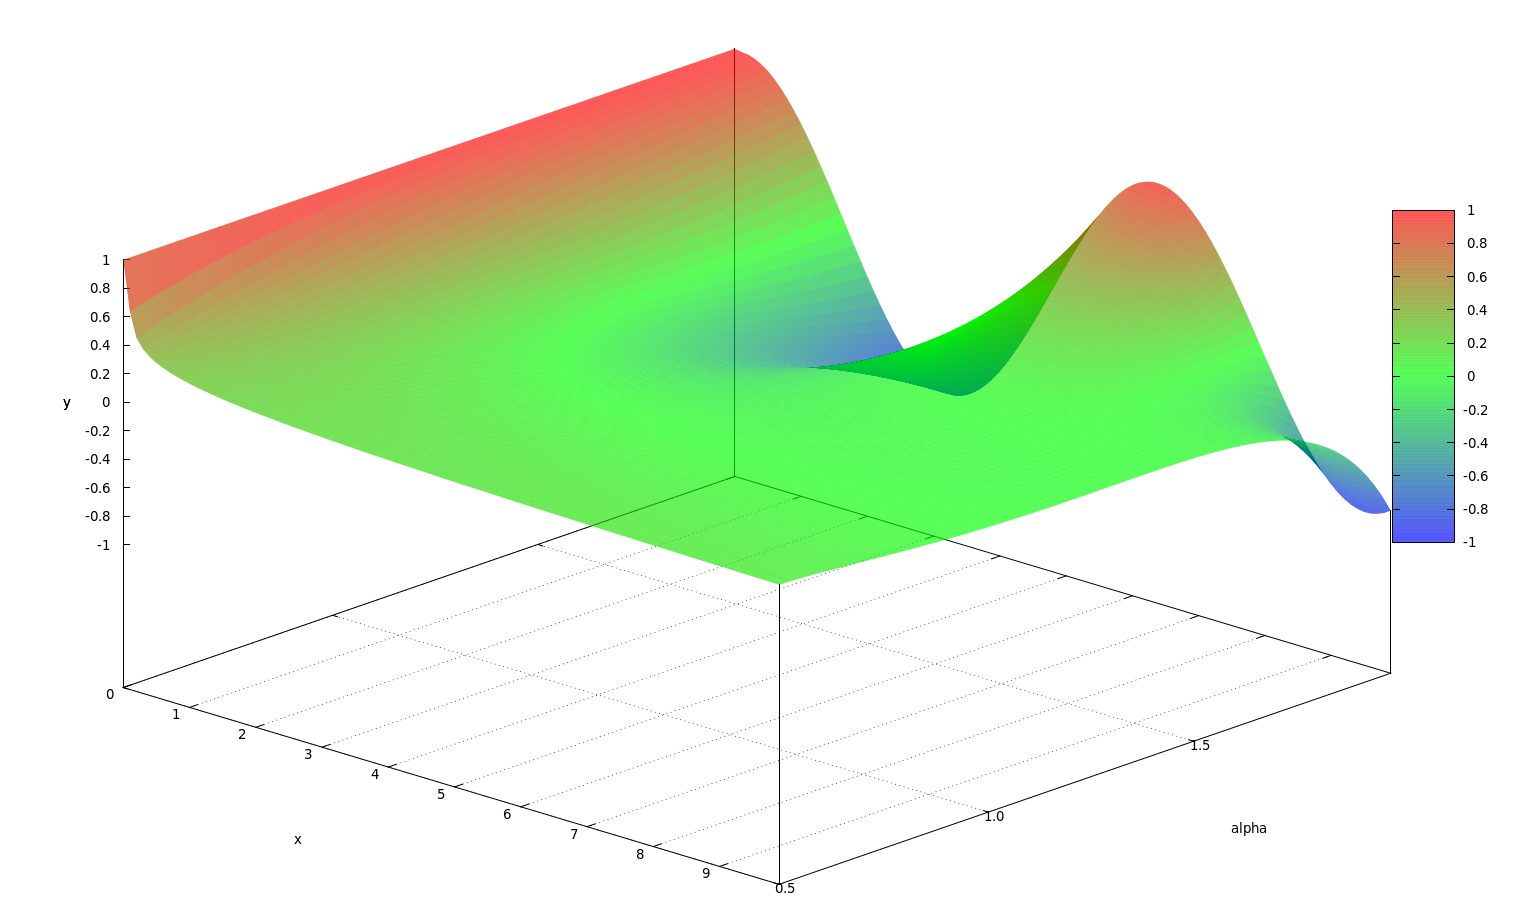
\includegraphics[scale = 0.2]{../images/FDE_Solution_Surface_No_Label}
\end{figure}
\end{frame}

\begin{frame}{Key references}
\begin{itemize}
\item [1] K. Diethelm. The Analysis of Fractional Differential Equations. Springer, 2010.

\item [2] K. Diethelm. An efficient parallel algorithm for the numerical solution of fractional differential equations. Fractional Calculus and Applied Analysis, 14:475–490, 2011.

\item [3] K. Diethelm, N.J. Ford, and A.D. Freed. Detailed error analysis for a fractional Adams method. Numerical
Algorithms, pages 31–52, 2004.
\end{itemize}
\end{frame}


\end{document}
